\documentclass[10pt]{exam}
\usepackage[icp]{template-for-exam}
\usepackage{hyperref,multicol,pgfplots}
\pgfplotsset{compat=1.18}

\title{Unit C1 Enrichment Activity}
\author{Rohrbach}
\date{\today}

\begin{document}
\maketitle

\noindent
This is an activity to work on {\bf when you are finished with everything we are doing in this unit}.  You can get 5 bonus points by completing this assignment at the end of the unit. However, you will not get any bonus if you have any missing assignments for the unit.  Other assignments are always more important than the Enrichment Activity!

\begin{questions}
  \question
    Go to the Density PhET Lab at \texttt{\href{https://phet.colorado.edu/en/simulations/density}{https://phet.colorado.edu/en/simulations/density}}.  Play with the simulation and write down three observations:
    \vs 

  \question
    Go to the ``Mystery'' tab.  Choose Block Set \#1.  Come up with a procedure to measure the density of each of these blocks, and explain your procedure below.
    \vs 

  \question
    Use your procedure to find the density of all the blocks in Block Set \#1.

    \begin{tabular}{|c|p{5em}|p{5em}||p{5em}|}
      \hline
      Block & Mass & Volume & Density \\\hline
      1A    &&&\\[1em]\hline
      1B    &&&\\[1em]\hline
      1C    &&&\\[1em]\hline
      1D    &&&\\[1em]\hline
      1E    &&&\\[1em]\hline
    \end{tabular}


  \pagebreak
  \question
    Go back to the ``Intro'' tab.  Pick wood plus two other materials (other than ``custom'').  Write down their densities in the data table below.  Then, move the volume slider up and down.  Write down the volume and mass for five different situations.  Make sure your five situations are spread out over the whole range of allowable volumes.


    \begin{multicols}{3}

      \paragraph{Material \#1:} Wood
    
      Density: \fillin[][7em]
  
      \begin{tabular}{|c|c|}
        \hline
        volume (L) & mass (kg) \\\hline
        1.00  &\\[1em]\hline
        3.00  &\\[1em]\hline
        5.00  &\\[1em]\hline
        7.00  &\\[1em]\hline
        10.00 &\\[1em]\hline
      \end{tabular}


      \paragraph{Material \#2:} \fillin[][5em]
    
      Density: \fillin[][7em]
  
      \begin{tabular}{|c|c|}
        \hline
        volume (L) & mass (kg) \\\hline
          &\\[1em]\hline
          &\\[1em]\hline
          &\\[1em]\hline
          &\\[1em]\hline
          &\\[1em]\hline
      \end{tabular}


      \paragraph{Material \#3:} \fillin[][5em]
    
      Density: \fillin[][7em]
  
      \begin{tabular}{|c|c|}
        \hline
        volume (L) & mass (kg) \\\hline
        &\\[1em]\hline
        &\\[1em]\hline
        &\\[1em]\hline
        &\\[1em]\hline
        &\\[1em]\hline
      \end{tabular}

    \end{multicols}

  \question
    Make a graph of the mass vs. volume for each of these materials.  Plot your points with dots.  Then connect the points with three different colors.

    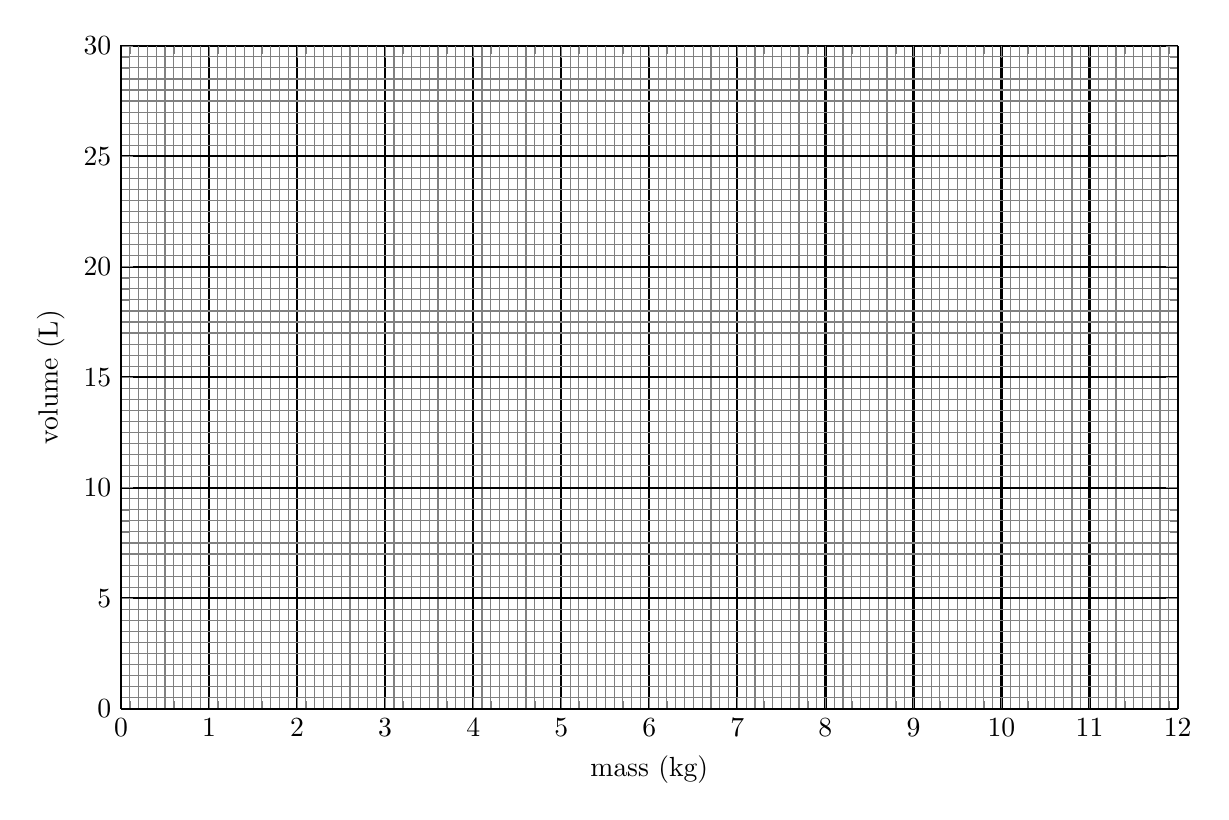
\begin{tikzpicture}
      \begin{axis}[
          xmin=0, xmax=12,
          ymin=0, ymax=30,
          width  = 15cm,
          height = 10cm,
          ylabel = {volume (L)},
          xlabel={mass (kg)},
          grid = both,
          minor tick num = 9,
          minor grid style = {gray,thin},
          major grid style = {black,thick},
      ]

      \end{axis}
    \end{tikzpicture}

  \question
    Draw some conclusions.  How does the graph of an object's mass and volume correspond to its density?
    \vs



\end{questions}



\end{document}